\documentclass[language=polish,type=master]{aghmodern}

\titleEN{Minimizing interaction delay in collaborative web applications}
\titlePL{Minimalizacja opóźnienia w interakcji użytkowników korzystających z aplikacji webowych}
\author{Piotr Szczygieł}
\faculty{Wydział Informatyki, Elektroniki i Telekomunikacji}
\department{Instytut Informatyki}
\supervisor{dr inż. Łukasz Czekierda}
\degreeprogramme{Informatyka}
\degreetype{Stacjonarne}
\date{2022}
\dedication{Test}

\usepackage[backend=biber,doi=true,url=false]{biblatex}
\addbibresource{bibliography.bib}

\usepackage[skip=2pt]{caption}

\setminted{autogobble,breaklines,frame=single,fontsize=\footnotesize}
\definecolor{number}{RGB}{102, 102, 102}
\definecolor{type}{RGB}{176, 0, 64}

\begin{document}

\frontmatter
\maketitle

\setcounter{tocdepth}{1}
\tableofcontents

\mainmatter

\onehalfspacing

\chapter{Wstęp}
Większość ludzi posiadających dostęp do Internetu każdego dnia korzysta z różnego rodzaju stron internetowych.
Kiedyś strony w większości były statyczne i nie wymagały od użytkownika żadnej interakcji.
Jednak wraz z rozwojem Internetu coraz więcej z nich zaczęła przekształcać się w interaktywne aplikacje webowe, umożliwiające użytkownikowi wchodzenie z nimi w interakcje oraz komunikacje z zewnętrznymi serwerami.
W kieszeni posiadamy komputery z procesorami szybszymi niż komputery personalne jeszcze nie tak dawno temu.
Pomimo tego aplikacje webowe w większości sprawiają wrażenie mało responsywnych i niewspółmiernie wolnych do sprzętu na którym są uruchamiane.
Na przestrzeni ostatnich lat pojawiły się technologie, których celem była adresacja tego problemu.
Jedną z nich był WebAssembly, który oferuje przeglądarkom środowisko uruchomieniowe dla programów kompilowanych.
Dzięki temu silniki przeglądarek mogłyby zaoszczędzić dużo czasu uruchamiając wcześniej skompilowane programy, zamiast interpretować i kompilować je w trakcie działania aplikacji.
Oprócz kwestii kodu wykonywanego lokalnie, dla większości interaktywnych aplikacji równie ważna jest komunikacja z zewnętrznymi serwerami.
Powszechnie używane technologie, takie jak ciągłe odpytywanie serwera (ang. polling) czy SSE\footnotemark{} nie umożliwiały uzyskanie dwukierunkowej, niskoopóźnieniowej komunikacji z serwerem.
\footnotetext{Server-sent events -- technologia umożliwiająca otrzymywanie wiadomości od serwera za pomocą połączenia HTTP}
Pojawienie się takich technologii jak WebRTC czy WebSocket, udostępniło aplikacjom webowym możliwość dwukierunkowej komunikacji z serwerem, bez stosowania protokołu HTTP nieprzystosowanego do takich zastosowań.
Praca ta skupi się na eksploracji tych technologii, które w założeniu powinny zmniejszyć opóźnienia użytkowników w interakcji z aplikacjami webowymi.

\section{Cel}
Celem pracy jest stworzenie zbioru rekomendacji dla programistów tworzących interaktywne aplikacje webowe.
Rekomendacje będą dotyczyć dwóch aspektów.
Pierwszym z nich będzie dobór technologii tworzenia aplikacji webowych, a konkretnie kwestia używania WebAssembly w nowych i istniejących aplikacjach.
Przedstawione zostaną przypadki, w których WebAssembly nie pomoże wydajności aplikacji.
Zaprezentowane zostaną również te, gdzie użycie WebAssembly znacząco poprawi wydajność i responsywność danej strony.
Rekomendacja będzie dotyczyć również wyboru języka programowania kompilowanego do WebAssembly.
Programista tworzący aplikację z użyciem WebAssembly, będzie musiał zdecydować się na język programowania, w którym będzie pracować.
Różnią się one między sobą wygodą użytkowania oraz wydajnością kodu wynikowego generowanego przez ich kompilatory, więc jest to również ważna decyzja.
Drugim aspektem jest wybór technologii komunikacji sieciowej.
Przedstawione zostaną wyniki testów opóźnień pomiędzy WebSocket, a WebRTC.
Oprócz tego przedstawione zostaną różnice w wygodzie tworzenia aplikacji z użyciem danej technologii.
Finalnie więc czytelnik będzie miał pogląd na technologie używane w procesie tworzenia wydajnych i responsywnych aplikacji webowych.

\section{Motywacja}
Pomimo wielkich postępów technologicznych w zakresie mocy obliczeniowej urządzeń z których korzystamy na co dzień, nadal mnóstwo stron internetowych potrafi ładować się po kilka sekund, a przy próbie interakcji z nimi zachowywać się nieresponsywnie.
Wiele osób jest poirytowanych takim stanem rzeczy i wspomina czasy dużo wolniejszych komputerów, na których aplikacje mimo tego ładowały się szybko i nie zacinały się.
Stan ten spowodowany jest w głównej mierze pewnego rodzaju chaosem panującym wśród twórców stron internetowych.
Poradniki do tworzenia nawet najprostszych aplikacji zawierają kod zaciągający tysiące bibliotek niepotrzebnie spowalniających ich działanie.
Nowoczesne technologie takie jak WebAssembly kuszą wielu programistów rozwiązaniem tych problemów.
Jednak aktualnie wiele programistów nadal nie jest do nich przekonana i rzadko wykorzystywane są one w aplikacjach, z którymi mnóstwo ludzi ma na co dzień do czynienia.
Aby ułatwić twórcom aplikacji wybór stosu technologicznego, skupiono się w tej pracy na przedstawieniu technologii usprawniających interaktywność aplikacji webowych.

\section{Metodyka}
Prace rozpoczęto od zapoznania się z językami kompilowanymi do WebAssembly.
Po wybraniu trzech interesujących języków utworzono z ich wykorzystaniem prosty benchmark.
Został on użyty do przeprowadzenia badań nad wydajnością aplikacji utworzonych w każdym z tych języków, a proces ich tworzenia dostarczył informacji o wygodzie pisania w danym języku.
Po wybraniu jednego z języków utworzono inne aplikacje webowe, które dostarczyły więcej informacji o danej technologii.
Pozwalały one zbadać wydajność aplikacji napisanej w tym języku i porównać ją z aplikacją napisaną w powszechnie stosowanym języku JavaScript.
Na koniec zaprojektowano przykładową interaktywną aplikacje webową.
Zostały utworzone trzy wersje aplikacji o identycznej funkcjonalności różniące się technologiami użytymi do jej stworzenia.
Utworzono aplikację webową JavaScript, aplikację webową korzystającą z WebAssembly oraz aplikację natywną.
Następnie wykonano testy porównujące technologie WebRTC oraz WebSocket w kontekście wykorzystania ich w takiej aplikacji.
Na podstawie otrzymanych wyników sporządzono wnioski oraz utworzono zestaw rekomendacji dla przyszłych programistów interaktywnych aplikacji webowych.

\section{Zawartość pracy}
Dalsza część pracy została rozdzielona na następujące części:

\begin{itemize}
    \item Rozdział 2 -- zawiera przedstawienie technologi WebAssembly oraz aktualnego stanu wiedzy na temat jej wydajności
    \item Rozdział 3 -- prezentuje technologie WebRTC i WebSocket wraz z aktualnym stanem wiedzy na ich temat
    \item Rozdział 4 -- przedstawia opis, analizę oraz porównanie języków kompilowanych do WebAssembly
    \item Rozdział 5 -- jest poświęcony dokładniejszej analizie wydajności aplikacji pisanych w języku programowania, który uzyskał najlepsze wyniki w poprzednim rozdziale
    \item Rozdział 6 -- prezentuje przykładową interaktywną aplikację webową umożliwiającą porównanie technologii WebRTC, WebSocket, WebAssembly i JavaScript wraz z rekomendacjami dotyczącymi ich wyboru
\end{itemize}

\chapter{WebAssembly}
W tym rozdziale przedstawiona zostanie technologia WebAssembly, jej zastosowania oraz aktualny stan wiedzy z nią związany.

\section{WebAssembly}
WebAssembly (w skrócie WASM) jest to binarny format instrukcji dla maszyny wirtualnej opartej na stosie.
Został stworzony jako przenośny cel kompilacji dla języków programowania\footnotemark{}.
\footnotetext{Aktualnie około 40 wysokopoziomowych języków programowania wspiera WebAssembly, m.in. C, C++, Python, Go, Java, PHP, Rust, Zig, AssemblyScript}
Umożliwia tworzenie aplikacji webowych działających zarówno po stronie klienta jak i serwera.

Maszyna WebAssembly została zaprojektowana do wczytywania binarnego formatu zapewniającego oszczędność rozmiaru i czasu ładowania uruchamianych na niej programów.
Celuje w osiągnięcie prędkości zbliżonej do natywnych aplikacji, korzystając z powszechnych możliwości sprzętowych\footnotemark{} dostępnych na różnych platformach.
\footnotetext{Przenośność WebAssembly wymaga, aby środowisko wykonywalne spełniało takie charakterystyki jak np. posiadanie 8 bitowych bajtów, możliwości adresowania pojedynczych bajtów pamięci, czy wykorzystanie IEEE 754 jako binarnej reprezentacji liczb zmiennoprzecinkowych}
Określa tzw. piaskownicę\footnotemark{}, czyli bezpieczne pod względem pamięci oraz dostępu z zewnątrz środowisko wykonywalne.
\footnotetext{Piaskownica (ang. sandbox) -- mechanizm izolacji uruchamianych programów służący poprawie bezpieczeństwa.}

Programy skompilowane do WebAssembly mogą być współcześnie stosowane jako dopełnienie JavaScript w tworzeniu aplikacji webowych.
Stopień tego dopełnienia może być różny, ale praca ta skupi się głównie na zastępowaniu fragmentów programu wykonujących dużą ilość obliczeń oraz wpływ tego na wydajność aplikacji.

Na listingu \ref{lst:wasm} poniżej zaprezentowano przykładową funkcję obliczającą silnie napisaną w języku C oraz wynik jej kompilacji do WebAssembly.
Jak można zauważyć wynikowy format WebAssembly jest bardzo zbliżony do języków asemblera, z których korzystają współczesne architektury, takie jak np. x86-64.
Upraszcza to bardzo zadanie silnikom przeglądarek, które tłumaczyć będą go na natywny kod maszynowy.

\begin{listing}[H]
\begin{center}
\begin{tabular}{ |p{0.3\textwidth}|p{0.3\textwidth}|p{0.3\textwidth}| }

\hline
Kod źródłowy C & Format tekstowy WASM & Format binarny WASM \\
\hline

\begin{minted}[frame=none,fontsize=\scriptsize]{c}
    int silnia(int n)
    {
     if (n == 0)
      return 1;
     else
      return n * silnia(n-1);
    }
\end{minted}

&

\begin{minted}[frame=none,fontsize=\scriptsize]{wat}
    (func (param i64)
          (result i64)
        local.get 0
        i64.eqz
        if (result i64)
            i64.const 1
        else
            local.get 0
            local.get 0
            i64.const 1
            i64.sub
            call 0
            i64.mul
        end)
\end{minted}

&

\begin{minted}[frame=none,fontsize=\scriptsize]{text}
    00 61 73 6D 01 00 00 00
    01 00 01 60 01 73 01 73 06
    03 00 01 00 02
    0A 00 01
    00 00
    20 00
    50
    04 7E
    42 01
    05
    20 00
    20 00
    42 01
    7D
    10 00
    7E
    0B
    0B 15 17
\end{minted}

\\

\hline

\end{tabular}
\end{center}

\caption{Porównanie kodu źródłowego funkcji oraz wynikowego kodu WebAssembly}
\label{lst:wasm}

\end{listing}

Aby użyć takiego skompilowanego modułu WebAssembly w aplikacji webowej należy go wczytać z poziomu języka JavaScript, co prezentuje kod poniżej.

\begin{listing}[H]
    \begin{minted}{javascript}
        const importObject = {
            module: {},
            env: {
                memory: new WebAssembly.Memory({ initial: 256 }),
            }
        };

        WebAssembly.instantiateStreaming(
            fetch("silnia.wasm"),
            importObject
        ).then(obj => {
            const silnia = obj.instance.exports.silnia;
            console.log(silnia(5));
        });
    \end{minted}
    \caption{Wczytanie i wywołanie funkcji z modułu WebAssembly}
\end{listing}

\section{Stan wiedzy}
Przedstawione poniżej prace poruszają kwestie porównania wydajności WebAssembly z resztą dostępnych rozwiązań.

W pracy \cite{wasm_blazor} \emph{Dawid Suryś}, \emph{Piotr Szłapa} oraz \emph{Maria Skublewska-Paszkowska} prowadzą badania nad wydajnością WebAssembly oraz JavaScript.
Dochodzą do wniosków, że WebAssembly może być szybszy od JavaScript w przypadku aplikacji zawierających dużą ilość obliczeń oraz operacji na zbiorach danych.
Mimo tworzenia aplikacji WebAssembly nadal jesteśmy zmuszeni do korzystania z JavaScript do wywoływania zapytań sieciowych czy operacji na DOM\footnotemark{}.
\footnotetext{Document Object Model -- sposób reprezentacji dokumentów HTML w postaci modelu obiektowego}
Powoduje to, że takie operacje są wolniejsze w WebAssembly niż w samym JavaScript przez dodatkowy narzut.
Przedstawiony test frameworka Blazor\footnotemark{} pokazał, że jest on wolniejszy niż istniejące popularne frameworki napisane w JavaScript.
\footnotetext{Blazor -- frontend w C\# wykorzystujący WebAssembly (\url{https://blazor.net/})}
Porównanie prędkości w tym przypadku jednak nie było do końca sprawiedliwe, ponieważ framework nie był bezpośrednio skompilowany do WebAssembly.
Był on skompilowany do kodu bajtowego platformy .NET, następnie uruchamianym w skompilowanym do WebAssembly CLR\footnotemark{}.
\footnotetext{Common Language Runtime -- środowisko uruchomieniowe dla platformy Microsoft .NET}
Pośrednio więc kod wykonywał się w dwóch zagnieżdżonych maszynach wirtualnych, co spowodowało jego mniejszą wydajność.
Projekt ten pokazał jednak, że WebAssembly jest na tyle dojrzały, aby stworzyć w nim kompletny i działający projekt.

Praca \cite{wasm_speedyjs} \emph{Micha Reiser} oraz \emph{Luc Bl\"{a}ser} przedstawia projekt \emph{Speedy.js}, który kompiluje wybrane funkcję z języka TypeScript\footnotemark{} do WebAssembly.
\footnotetext{TypeScript -- statycznie typowany nadzbiór JavaScript (\url{https://www.typescriptlang.org/})}
Generuje on również automatycznie kod pozwalający na łatwą integrację z resztą kodu napisanego w TypeScript.
W niektórych przypadkach osiągnięto nawet czterokrotne przyspieszenie dla funkcji skompilowanych do WebAssembly.
Projekt proponuje ciekawą strategię stopniowej transformacji kodu obliczeniowo intensywnego do WebAssembly.

\emph{Abhinav Jangda} i inni w swojej pracy \cite{wasm_native} porównują wydajność WebAssembly z natywnymi aplikacjami.
Wykorzystując \emph{BROWSIX-WASM}\footnotemark{} porównano wydajność programów skompilowanych do aplikacji natywnych oraz WebAssembly.
\footnotetext{BROWSIX -- projekt umożliwiający uruchamianie niezmodyfikowanych plików wykonywalnych systemu Linux w przeglądarce (\url{https://browsix.org/})}
Aplikacje WebAssembly były średnio wolniejsze od natywnych aplikacji o 1.55x dla przeglądarki Chrome i 1.45x dla Firefox.
Główny powód dla którego WebAssembly jest wolniejsze od natywnej aplikacji to gorsza optymalizacja kodu maszynowego.
Spowodowane jest to ograniczeniami wynikającymi ze specyfikacji WebAssembly (np. stack overflow checks, indirect call checks, reserved registers).
Ograniczenia te nie muszą być zawarte w aplikacji natywnej.

Artykuł \cite{wasm_js_bench} napisany przez \emph{David Herrera} i innych zawiera zbiór benchmarków porównujących WebAssembly oraz JavaScript w różnych konfiguracjach.
Dla maszyny z systemem Windows, WebAssembly był około 70\% szybszy dla przeglądarki Chrome, 60\% szybszy dla Firefox i 163\% szybszy dla przeglądarki Edge.
Z tych trzech przeglądarek najlepsze wyniki odniósł Firefox.

\emph{Weihang Wang} w swoim artykule \cite{wasm_js_bench2} porównuje WebAssembly i JavaScript dla czasu wykonania i zużycia pamięci różnych programów.
Zauważa, że WebAssembly zużywa dużo więcej pamięci niż JavaScript.
Mimo tego WebAssembly był dużo szybszy od JavaScript dla bardzo małych rozmiarów danych (35.3x średnie przyspieszenie) oraz małych danych (7.67x średnie przyspieszenie).
Natomiast dla większych rozmiarów danych, dzięki \emph{JIT}\footnotemark{}, JavaScript doganiał WebAssembly, a nawet zdarzały się przypadki gdzie WebAssembly był wolniejszy od JavaScript.
\footnotetext{Kompilator JIT -- kompiluje kod w trakcie wykonywania programu, w przeciwieństwie do zwykłych kompilatorów, które robią to przed jego uruchomieniem}
Otrzymane przez niego wyniki pokazują, że optymalizacja \emph{JIT} w Chrome znacząco poprawia wyniki JavaScript, nie mając wpływu na WebAssembly.

\section{Wnioski}
WebAssembly jest obiecującą technologią.
Dla wielu przypadków osiągał dużo lepsze wyniki, jeśli chodzi o obliczenia w przeglądarce.
Mimo tego wspomniane prace głównie skupiały się na samej wydajności, a niewiele było poruszonych tematów tworzenia aplikacji.
Wiele benchmarków były to programy napisane w C przeportowane\footnotemark{} do WebAssembly.
\footnotetext{Portowanie -- proces przenoszenia wersji programu komputerowego na inną platformę sprzętową lub programistyczną}
W tej pracy poruszony zostanie natomiast temat tworzenia nowych aplikacji oraz wybór języka kompilowanego do WebAssembly, który się do tego najbardziej aktualnie nadaje.

\chapter{WebRTC i WebSocket}
W tym rozdziale zaprezentowane zostaną technologie WebRTC i WebSocket oraz aktualny stan wiedzy z nimi związany.

\section{WebRTC}
WebRTC to otwartoźródłowy projekt zapewniający przeglądarkom internetowym możliwość komunikacji w czasie rzeczywistym za pomocą zestawu interfejsów programowania.
Umożliwia aplikacjom webowym przechwytywanie oraz opcjonalne strumieniowanie mediów audio-wizualnych.
Pozwala również na wymianę różnorodnych danych pomiędzy przeglądarkami bez konieczności posiadania serwera pośredniczącego.
Pod spodem korzysta z protokołów UDP, TCP oraz SCTP w zależności od ustawień firewall użytkowników oraz rodzaju przesyłanych danych.

Udostępniony zestaw interfejsów programowania dla języka JavaScript to między innymi:

\begin{itemize}
    \item \emph{getUserMedia} -- otrzymuje dostęp do mediów audio-wizualnych użytkownika (np. uzyskując dostęp do mikrofonu oraz kamery)
    \item \emph{RTCPeerConnection} -- uruchamia komunikacje audio-wizualną pomiędzy użytkownikami, odpowiada za przetwarzanie sygnału, obsługę kodeków, komunikację, bezpieczeństwo oraz zarządzanie prędkości połączenia
    \item \emph{RTCDataChannel} -- umożliwia dwukierunkową komunikacje z wykorzystaniem różnorodnych danych pomiędzy użytkownikami
\end{itemize}

Interfejs programowania WebRTC nie udostępnia możliwości wykrywania innych użytkowników do których można się połączyć.
W większości aplikacji rozwiązane jest to za pomocą zewnętrznego serwera sygnalizującego, który umożliwia wymianę kandydatów ICE\footnotemark{}.
\footnotetext{Interactive Connectivity Establishment -- technika umożliwiająca znalezienie sposobu komunikacji użytkowników w najbardziej bezpośredni sposób}
Użytkownicy znajdujący się z NATem będą musieli również skomunikować się z serwerem STUN\footnotemark{}, w celu otrzymania swojego publicznego adresu IP.
\footnotetext{Session Traversal Utilities for NAT -- protokół sieciowy pozwalający klientom ukrytym za NAT na znalezienie ich publicznych adresów IP}
W przypadku braku możliwość ustanowienia bezpośredniej komunikacji będzie konieczne również skorzystanie z pośredniczącego serwera TURN\footnotemark{}, którego jedynym zadaniem jest przekazywanie wiadomości pomiędzy klientami.
\footnotetext{Traversal Using Relays around NAT -- protokół służący do przekazywania ruchu sieciowego umożliwiający komunikacje, kiedy nie jest możliwe ustanowienie bezpośredniego połączenia}
Rysunek \ref{fig:webrtc} poniżej przedstawia ten proces inicjalizacji połączenia pomiędzy dwoma użytkownikami.

\begin{figure}[H]
    \centering
    \vspace*{15pt}
    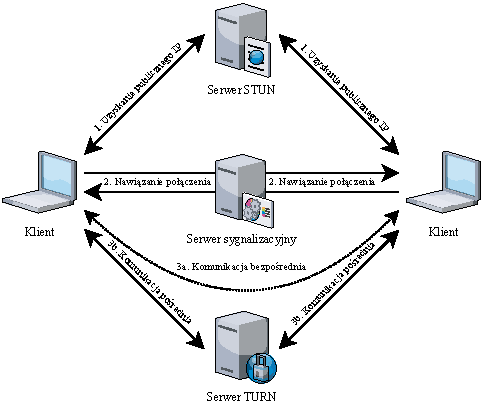
\includegraphics[width=\textwidth]{images/webrtc.pdf}
    \caption{Komunikacja z wykorzystaniem technologii WebRTC}
    \label{fig:webrtc}
\end{figure}

\section{WebSocket}
WebSocket natomiast to technologia umożliwiająca otwarcie interaktywnej sesji komunikacji pomiędzy przeglądarką a serwerem.
Zapewnia dwukierunkowy kanał wymiany danych poprzez pojedyncze połączenie TCP.
Przedstawione poniżej prace skupiają się na porównaniu tych dwóch technologii w różnych kontekstach.

\section{Stan wiedzy na temat WebRTC i WebSocket}
\emph{G{\"u}nay Mert Karadogan} w swojej pracy \cite{websocket_webrtc_iot} bada WebRTC oraz WebSocket pod względem użycia ich w IoT\footnotemark{}.
\footnotetext{Internet of Things -- sieć fizycznych obiektów wyposażonych w czujniki i oprogramowanie umożliwiające wymianę danych z innymi urządzeniami za pośrednictwem Internetu}
Wnioskuje on, że zarówno WebSocket jak i WebRTC może zostać użyte do łączenia urządzeń IoT z Internetem.

\emph{Tomasz Karla} i \emph{Jarosław Tarnawski} w pracy \cite{websocket_webrtc_realtime} porównują opóźnienie technologii WebRTC oraz WebSocket w różnych scenariuszach.
Testowane były przykładowo sieci lokalne, GSM oraz WiFi. Technologia WebRTC zanotowała minimalnie mniejsze opóźnienia.
Umożliwił on również komunikacje aplikacji w obrębie sieci lokalnej\footnotemark{}, mimo postawienia strony na publicznym serwerze.
\footnotetext{WebRTC potrafi połączyć się między dwoma przeglądarkami bezpośrednio, jeśli ustawienia Firewall użytkowników na to pozwalają}
Autorzy wnioskują, że obie technologie jak najbardziej nadają się do tworzenia aplikacji sieciowej.

Praca \cite{websocket_webrtc_streamr} \emph{Santeri Juslenius} analizowała zachowanie technologii WebRTC oraz WebSocket w sieci \emph{Streamr}, która jest zdecentralizowanym systemem \emph{publish-subscribe}\footnotemark{}.
\footnotetext{Jest to system komunikacji, w którym wysyłane wiadomości mają przypisane pewne kategorie, które odbiorcy mogą subskrybować w celu ich otrzymywania}
Na podstawie wyników badań autorzy doszli do wniosku, że WebSocket odnosi lepsze rezultaty pod względem opóźnień.
Jednak dla tej konkretnej topologii WebRTC był bardziej użyteczny ze względu na lepsze wyniki dla małych pakietów oraz możliwości połączeń P2P.

\section{Wnioski}
Wszystkie prace zgodnie uznają, że obie technologie nadają się do tworzenia aplikacji sieciowych.
Niektóre mówią o niższych opóźnieniach dla WebRTC, a inne dla WebSocket.
W tej pracy porównamy wykorzystanie tych technologii w interaktywnych aplikacjach webowych.

\chapter{Języki kompilowane do WebAssembly}
WebAssembly jest binarnym formatem, interpretowanym przez wirtualną maszynę uruchamianą w przeglądarce lub jako niezależną aplikację.
Nie jest on więc językiem programowania samym w sobie.
Może on natomiast być celem kompilacji dla innych języków.
Wybór takiego języka może okazać się równie ważny jak podjęcie decyzji o tym czy w ogóle korzystać z WebAssembly.
Aktualnie dużo języków ma możliwość ustawienia WebAssembly jako platformę wynikową kompilacji.
W tej pracy jednak skupiono się na trzech: Zig, AssemblyScript oraz Rust.
Pierwszym językiem, któremu zostanie poświęcona uwaga w tej pracy jest Zig.
Jest to młody, szybko rozwijający się język, którego celem jest zastąpienie współczesnych użyć języka C.
AssemblyScript został wybrany jako język bardzo zbliżony składnią i użyciem do popularnego TypeScript.
Dzięki niemu programiści stron internetowych mogliby bez dużej ilości nauki tworzyć moduły WebAssembly.
Rust został wybrany ze względu na największą popularność wśród programistów WebAssembly.
W tym rozdziale przedstawione będzie porównanie tych języków zarówno pod względem wydajności kodu wynikowego jak i prostoty tworzenia aplikacji.
Pominięto takie języki jak C oraz C++ ze względu na to, że tak samo jak Rust i Zig korzystają z LLVM\footnotemark{} do generowania kodu wynikowego.
\footnotetext{LLVM -- backend dla kompilatorów z którego korzystają różne frontendy dla takich języków jak C, C++, Rust, Zig, Swift i wiele innych (\url{https://llvm.org/})}
Z tego powodu różnice w wydajności kodu wynikowego będą marginalne i będą wywodzić się głównie ze stylu pisania kodu w danym języku.
Mimo, że pod spodem korzystają z tego samego kompilatora, to programy napisane w języku C często są szybsze od ich odpowiedników w C++.
Spowodowane jest to tym, że programiści C pozbawieni takich funkcjonalności języka jak RAII\footnotemark{}, zmuszeni są do bardziej szczegółowej kontroli alokacji pamięci i sposobu ułożenia w niej danych.
\footnotetext{Resource acquisition is initialization -- wzorzec projektowy łączący konstrukcję i destrukcję obiektu z alokacją i zwalnianiem zasobów z których korzysta}
Z tego powodu C i C++ niekoniecznie będą wydajniejsze od Rust, a współcześnie programiści starają się odchodzić od korzystania z tych języków w nowych projektach na rzecz nowocześniejszych i wygodniejszych technologii.
Zaprezentowane zostanie utworzenie dwóch prostych funkcji w każdym z języków -- rekurencyjnego obliczania n-tej liczby ciągu Fibonacciego oraz sortowania tablicy liczb.
Proces ich implementacji będzie służył zaobserwowaniu jak skomplikowane jest utworzenie modułu WebAssembly w każdym z wybranych języków.
Przedstawiona będzie rekurencyjna wersja obliczania n-tej liczby ciągu Fibonacciego zamiast iteracyjnej, ponieważ jest dużo wolniejsza i szybko zapełnia stos, dzięki czemu łatwiej pokazuje różnice w wydajności między językami.
Te dwie testowane funkcje nie umożliwią dokładnego porównania wydajności kodu wynikowego dla tych języków, ale zapewnią nam pewien powierzchowny wgląd w ich wydajność, który wystarczy do wstępnej oceny danego języka.

\section{Zig}
Posiłkując się definicją ze strony głównej projektu\footnotemark{}, Zig to język programowania ogólnego przeznaczenia i zestaw narzędzi do utrzymywania solidnego i optymalnego oprogramowania wielokrotnego użytku.
\footnotetext{\url{https://ziglang.org/}}
Jest nowoczesnym zastępcą języka C, czyli niskopoziomowym kompilowanym językiem, bez ukrytych alokacji pamięci, automatycznej dezalokacji i tym podobnych rozwiązań.
Jednocześnie próbuje naprawić główne problemy swojego poprzednika przykładowo wychwytując dużo problemów związanych z bezpieczeństwem pamięci już w trakcie kompilacji.

\subsection{Instalacja}
Proces instalacji potrzebnych narzędzi jest bardzo prosty i zajmuje dosłownie minutę.
Wystarczy pobrać archiwum ze strony, wypakować i ewentualnie dodać folder do zmiennej środowiskowej \emph{PATH}, aby można było kompilować bez podawania pełnej ścieżki do kompilatora.
Zamiast pobierać manualnie, można też skorzystać z menadżera paczek dla używanego systemu operacyjnego.
Pobrany zestaw narzędzi zawiera wszystko co potrzebne do utworzenia modułu WebAssembly.

\subsection{Tworzenie funkcji \emph{fib}}
Tworzenie aplikacji można rozpocząć od napisania funkcji rekurencyjnie liczącej n-tą liczbę w ciągu Fibonacciego.

\begin{listing}[H]
    \begin{minted}{zig}
        export fn fib(n: u64) u64 {
            if (n == 1) return 1;
            if (n == 2) return 1;
            return fib(n - 1) + fib(n - 2);
        }
    \end{minted}
    \caption{Funkcja \emph{fib} w języku Zig}
\end{listing}

Jak widać składnia jest bardzo zbliżona do języków z rodziny C.
Słowo kluczowe \emph{export} umożliwia wywołanie danej funkcji z poziomu JavaScript.

\subsection{Tworzenie funkcji \emph{sort}}
Kolejnym krokiem jest utworzenie funkcji, która otrzymuje tablicę z zewnątrz, a następnie ją sortuje.
Pojawia się tutaj jednak pierwszy problem -- zarządzanie pamięcią.
Nie można mianowicie przekazać tablicy bezpośrednio z poziomu kodu napisanego w JavaScript do modułu WebAssembly.
Program napisany w Zig ma jedynie dostęp do swojej pamięci, która znajduję się w piaskownicy.
Należy więc udostępnić tę pamięć użytkownikowi, aby mógł przez nią przekazać nam tablicę do posortowania.

% Minted doesn't detect Zig 10_000_000 number correctly and it breaks syntax highlighting
\begin{listing}[H]
    \begin{minted}[escapeinside=||]{zig}
        const std = @import("std");
        const allocator = @import("std").heap.page_allocator;

        var array: []f64 = undefined;

        export fn initialize_array() *f64 {
            array = allocator.alloc(f64, |\textcolor{number}{10\_000\_000}|) catch unreachable;
            return &array[0];
        }

        export fn sort(size: usize) void {
            std.sort.sort(f64, array[0..size], {}, comptime std.sort.asc(f64));
        }
    \end{minted}
    \caption{Funkcja \emph{sort} i jej kod pomocniczy w języku Zig}
\end{listing}

Funkcja \emph{initialize\_array} alokuje najpierw 10MB pamięci, a następnie zwraca wskaźnik na początek zaalokowanej tablicy.
Dzięki temu użytkownik będzie mógł ją wypełnić swoimi danymi, a następnie za pomocą funkcji \emph{sort} posortować N pierwszych liczb.
Nie jest to najwygodniejszy sposób pisania kodu operującego na danych przekazywanych z poziomu strony internetowej.
Aby dało się w prostszy sposób przekazywać dane należałoby zaimplementować swój własny alokator\footnotemark{} pamięci WebAssembly.
\footnotetext{Alokator -- odpowiada za zarządzanie dynamiczną pamięcią programu, czyli jej alokacje, dezalokacje i realokacje}
Za jego pomocą przed wywołaniem funkcji z poziomu JavaScript można by przekopiować dane o konkretnym rozmiarze do pamięci WebAssembly.
Istnieje wprawdzie gotowy alokator \emph{zee\_alloc}\footnotemark{}, ale problemy z jego wdrożeniem do projektu, brak dokumentacji oraz mała popularność spowodowały zaniechanie próby wykorzystania go w testach.
\footnotetext{\url{https://github.com/fengb/zee_alloc}}
Inne języki zaprezentowane w tej pracy posiadają swoje własne implementacje alokatorów oraz funkcjonalność generowania kodu pomocniczego.
Problem ten więc nie występuje w ich przypadku.

\subsection{Kompilacja}
Można teraz skompilować plik, który nazwany został \emph{main.zig} i utworzyć moduł WebAssembly \emph{zig.wasm} następującym poleceniem:

\begin{minted}{console}
    $ zig build-lib main.zig -target wasm32-freestanding -dynamic -O ReleaseFast -femit-bin=zig.wasm
\end{minted}

Ustawiono poziom optymalizacji na \emph{ReleaseFast}, aby uzyskać jak najlepszą wydajność modułu.
Język Zig oprócz kompilacji z poziomu linii poleceń umożliwia również tworzenie bardziej skomplikowanych programów budujących.
Mogą być one napisane również w języku Zig, zamiast w jakimś innym, nie związanym z aplikacją języku opisującym proces budowania.
Dzięki temu nie trzeba uczyć się dodatkowych narzędzi takich jak CMake, Make czy wiele innych.
Temat ten jednak wychodzi poza zakres tej pracy.

\section{AssemblyScript}
AssemblyScript został zaprojektowany specjalnie dla WebAssembly.
Dzięki temu nie musimy korzystać z dodatkowych bibliotek, aby umożliwić jego kompilację do WebAssembly.
Korzysta ze składni bardzo zbliżonej do języka TypeScript, dzięki czemu programiści stron internetowych nie muszą poświęcać dużo czasu na jego naukę.

\subsection{Instalacja}
AssemblyScript w prosty sposób integruje się z istniejącym ekosystemem stron internetowych.
Zainstalować go można korzystając z menadżera paczek \emph{npm}.
Cały proces inicjalizacji nowego projektu jest szybki, prosty i dokładnie opisany w oficjalnym wstępie do języka\footnotemark{}.
\footnotetext{\url{https://www.assemblyscript.org/getting-started.html}}

\subsection{Tworzenie funkcji \emph{fib}}
Pisanie kodu rozpoczęto w wygenerowanym pliku \emph{index.ts} od funkcji \emph{fib}.

% Second u64 is not highlighted for some reason
\begin{listing}[H]
    \begin{minted}[escapeinside=||]{typescript}
        export function fib(n: u64): |\textcolor{type}{u64}| {
            if (n == 1) return 1;
            if (n == 2) return 1;
            return fib(n - 1) + fib(n - 2);
        }
    \end{minted}
    \caption{Funkcja \emph{fib} w języku AssemblyScript}
\end{listing}

Kod jest praktycznie taki sam jaki można by napisać w języku TypeScript.
Główną różnicą jest użycie typu \emph{u64}, ponieważ WebAssembly wymaga specyfikacji konkretnego typu liczby obsługiwanego przez maszynę wirtualną.

\subsection{Tworzenie funkcji \emph{sort}}

Funkcje sort można w tym języku napisać dużo szybciej niż w języku Zig.

\begin{listing}[H]
    \begin{minted}{typescript}
        export function sort(array: Array<f64>): void {
            array.sort();
        }
    \end{minted}
    \caption{Funkcja \emph{sort} w języku AssemblyScript}
\end{listing}

Jak można zauważyć, wystarczy że ustawimy typ zmiennej wejściowej jako \emph{Array<f64>}, aby funkcja przyjmowała tablicę liczb zmiennoprzecinkowych.
W przeciwieństwie do języka Zig, nie jest konieczne manualnie tworzenie bufora, do którego przekażemy tablice z zewnątrz.
AssemblyScript w trakcie kompilacji automatycznie generuje kod, dzięki któremu nie musimy się tym przejmować.
Tworzona jest funkcja okalająca (ang. wrapper function), która alokuje pamięć dla naszej tablicy i przekazuje ją do właściwej funkcji jako wskaźnik na tę pamięć.

\subsection{Kompilacja}
Skompilować projekt możemy za pomocą narzędzia \emph{npm}.

\begin{minted}{console}
    $ npm run build
\end{minted}

Podczas inicjalizacji projektu wygenerowały się pliki konfiguracyjne, które powodują, że to polecenie kompiluje program do modułu WebAssembly.
Co ważne w przypadku tego języku, z racji na ścisłą integrację z resztą ekosystemu tworzenia stron internetowych, buduje to również jednocześnie pozostały kod strony.
Oznacza to, że nie potrzebujemy dodatkowego kroku kompilacji WebAssembly, a wszystko odbywa się z użyciem jednego systemu budującego.
Bardzo przydatną funkcją są również automatycznie generowane pliki typów TypeScript.

\begin{listing}[H]
    \begin{minted}{typescript}
        export declare function fib(n: bigint): bigint;
        export declare function sort(array: Array<number>): void;
    \end{minted}
    \caption{Fragment wygenerowanego pliku typów AssemblyScript}
\end{listing}

Dzięki nim otrzymywano podpowiedzi w środowisku programistycznym w trakcie odwoływania się do funkcji napisanych w AssemblyScript.

\section{Rust}
Rust, podobnie jak Zig jest językiem programowania ogólnego przeznaczenia.
Stworzony został z myślą o bezpieczeństwie, współbieżności i praktyczności.
Według corocznej ankiety serwisu Stack Overflow\footnotemark{}, Rust jest najbardziej lubianym językiem programowania od 2015 roku.
\footnotetext{\url{https://insights.stackoverflow.com/survey/}}

\subsection{Instalacja}
Rust można zainstalować korzystając z menadżera paczek systemu operacyjnego lub skorzystać z programu \emph{rustup}\footnotemark{}, który szybko przeprowadzi użytkownika przez kolejne kroki instalacji.
\footnotetext{\url{https://rustup.rs/}}
Instalacja w systemie Windows wymaga również zainstalowania Microsoft Visual Studio dla języka C++.
Po zainstalowaniu języka możemy przystąpić do tworzenia nowego projektu.
Książka \emph{Rust and WebAssembly}\footnotemark{} prezentuje krok po kroku ten proces.
\footnotetext{\url{https://rustwasm.github.io/}}
Jest on prosty i zrozumiały oraz przedstawia jak w prosty sposób zintegrować utworzone moduły ze stronami internetowymi.

\subsection{Tworzenie funkcji \emph{fib}}
Po przygotowaniu środowiska można rozpocząć edycję pliku \emph{lib.rs}.

\begin{listing}[H]
    \begin{minted}{rust}
        #[wasm_bindgen]
        pub fn fib(n: u64) -> u64 {
            match n {
                1 => 1,
                2 => 1,
                _ => fib(n - 1) + fib(n - 2)
            }
        }
    \end{minted}
    \caption{Funkcja \emph{fib} w języku Rust}
\end{listing}

Jak widać, poza specyficzną dyrektywą \emph{match}, kod powinien być zrozumiały dla większości programistów.
W języku Rust ostatnie wyrażenie w funkcji uznawane jest jako wartość zwracana, a dyrektywa \emph{match} działa podobnie jak \emph{switch} w językach z rodziny C.
Atrybut \emph{wasm\_bindgen} oznacza funkcje jako dostępną do wywołania z poziomu kodu JavaScript strony internetowej.
Jest to wymagane, dlatego że oprócz modułu WebAssembly, automatycznie generowany będzie również kod JavaScript inicjalizujący ten moduł oraz dodający funkcje pomocnicze.
Podobne rozwiązanie mogliśmy zauważyć w projekcie AssemblyScript, a brak jego jest odczuwalny tworząc projekt w języku Zig.

\subsection{Tworzenie funkcji \emph{sort}}
Przekazywanie tablicy do modułu WebAssembly można zrobić na różne sposoby.
Jeden z nich jest przedstawiony poniżej.

\begin{listing}[H]
    \begin{minted}{rust}
        #[wasm_bindgen]
        pub fn sort(js_array: &Float64Array) {
            let mut numbers: Vec<f64> = js_array.to_vec();
            numbers.sort_by(|a, b| a.partial_cmp(b).unwrap());
        }
    \end{minted}
    \caption{Funkcja \emph{sort} w języku Rust}
\end{listing}

Przekazaną z poziomu JavaScript tablicę konwertujemy na natywny dla języka Rust typ \emph{Vec}, który określa dynamiczną tablicę.
Może to spowodować mały narzut czasowy, ale jeśli byłoby to konieczne, można podobnie jak w języku Zig, udostępnić bezpośrednio adres pamięci do zapisu.
Rozwiązanie tutaj przedstawione jest jednak preferowane w większości wypadków, ponieważ programista nie musi się zastanawiać nad zarządzaniem pamięcią udostępnianą przeglądarce.
Po konwersji tablicy na typ \emph{Vec} używamy na niej funkcji \emph{sort\_by}, która sortuje tablicę.

\subsection{Kompilacja}
Cały projekt kompilujemy korzystając z programu \emph{wasm-pack}.

\begin{minted}{console}
    $ wasm-pack build
\end{minted}

Kompilator, podobnie jak w przypadku AssemblyScript, oprócz utworzenia samego modułu WebAssembly, generuje również pomocnicze funkcje JavaScript oraz pliki typów TypeScript.
Generowane są również funkcje okalające, które alokują pamięć dla tablicy i przekazują ją pod spodem do właściwej funkcji.

\section{Porównanie języków}
Każdy z przedstawionych języków różnił się od pozostałych pod wieloma względami.
Bezpośrednie stwierdzenie, który z nich jest lepszy lub gorszy nie jest do końca możliwe.
Można natomiast porównać je pod względem wydajności oraz prostoty użytkowania i na tej podstawie stwierdzić, który z nich będzie rozsądnym wyborem dla większości osób.

\subsection{Instalacja}
Pod względem instalacji najwygodniejszy zdecydowanie był język Zig.
Instalacja sprowadzała się do pobrania i wypakowania archiwum, po czym można było rozpocząć tworzenie projektu.
AssemblyScript oraz Rust były trochę cięższe w instalacji, ale nie były one też specjalnie trudne.
Instalacja trwała po prostu dłużej.
Należy też zaznaczyć, że projekty tworzone w AssemblyScript oraz Rust, oprócz kompilacji do modułu WebAssembly, generowały też przydatne pliki JavaScript oraz TypeScript.
Zig na dzień dzisiejszy nie posiada bibliotek, które umożliwiałyby taką funkcjonalność.

\subsection{Implementacja prostych funkcji}
Kwestia składni i prostoty pisania w danym języku jest bardzo subiektywna, ponieważ w zależności od umiejętności i doświadczenia, każda osoba może mieć inne odczucia.
Najbardziej wyróżniającym się problemem były trudności w przekazywaniu dużych tablic do funkcji napisanej w języku Zig.
Zarówno Rust jak i AssemblyScript, dzięki generowaniu pomocniczych modułów JavaScript odciążają programistę z konieczności implementacji ich samemu.
Bardzo ważną kwestią jest też to, że Zig nie posiada żadnego wsparcia dla integracji z aplikacjami internetowymi.
Rust i AssemblyScript generując wspominane wcześniej pomocnicze moduły, bardzo upraszczają integrację modułu WebAssembly z resztą kodu pisanego w JavaScript.

\subsection{Wydajność}
Jednym z najważniejszych zagadnień w kontekście minimalizacji opóźnień aplikacji jest wydajność programów napisanych w danym języku.
W celu dokonania porównania, utworzono prostą aplikacje internetową.
Ładuje ona stworzone wcześniej moduły WebAssembly i wypisuje czas wywołania konkretnych funkcji dla różnych parametrów.
Warto też wspomnieć, że wyniki zależą od użytego sprzętu oraz przeglądarki.
Wszystkie aplikacje uruchamiane były na przeglądarce Google Chrome\footnote{\url{https://www.google.com/chrome/}} oraz Mozilla Firefox\footnote{\url{https://www.mozilla.org/firefox/}}.
Konfiguracja sprzętowa komputera testowego przedstawia się następująco:
\begin{itemize}
    \itemsep0em
    \item Procesor \emph{ADM Ryzen 5 5600} -- 6 rdzeni / 12 wątków / 4,4 GHz
    \item Karta graficzna \emph{GeForce GTX 1080}
    \item Pamięć RAM 16GB DDR4
    \item System operacyjny \emph{Windows 10}
\end{itemize}

Poniżej przedstawiono również kod w języku JavaScript do którego porównywane były inne wyniki.

\begin{listing}[H]
    \begin{minted}{javascript}
        function sort(array) {
            array.sort();
        }

        function fib(n) {
            if (n === 1) return 1;
            if (n === 2) return 1;
            return fib(n - 1) + fib(n - 2); 
        }
    \end{minted}
    \caption{Funkcje \emph{sort} oraz \emph{fib} zaimplementowany w języku JavaScript}
\end{listing}

Analizę wydajności rozpoczęto od funkcji sortującej milion liczb.
Jak można zauważyć na wykresie \ref{fig:sort6}, aplikacje stworzone w Rust i Zig osiągnęły najlepsze wyniki, AssemblyScript był od nich trochę wolniejszy.
Dla przeglądarki Chrome wszystkie moduły WebAssembly były o cały rząd złożoności szybsze niż JavaScript.
Dla przeglądarki Firefox natomiast Zig i Rust były około czterokrotnie szybsze, a AssemblyScript około dwukrotnie szybszy.

\begin{figure}[H]
    \centering
    \import{plots}{sort6.pgf}
    \caption{Czasy sortowania miliona liczb}
    \label{fig:sort6}
\end{figure}

Dla funkcji obliczającej ciąg Fibonacciego, w przypadku przeglądarki Firefox odnotowano podobne zależności jak w poprzednim teście.
Na wykresie \ref{fig:fib40} można zauważyć, że najgorszy wynik uzyskała zwykła funkcja JavaScript.
Aplikacje napisane w Rust i Zig odnotowują najlepsze wyniki, natomiast AssemblyScript jest od nich trochę wolniejsze.
W przeglądarce Chrome natomiast sytuacja przedstawia się trochę inaczej.
Na wykresie \ref{fig:fib40} można zauważyć, że najgorszy wynik uzyskało AssemblyScript.
Rust jest tylko trochę szybszy od JavaScript, a Zig jest prawie dwukrotnie szybszy niż Rust.

\begin{figure}[H]
    \centering
    \import{plots}{fib40.pgf}
    \caption{Czasy wykonania \emph{fib(40)}}
    \label{fig:fib40}
\end{figure}

\section{Wnioski}
Biorąc pod uwagę, że dla tematu tej pracy wydajność ma największe znaczenie, to AssemblyScript nie do końca jest w stanie konkurować z językami Rust i Zig.
Jakikolwiek wynik gorszy niż JavaScript świadczy o tym, że może kompilatorowi brakować niektórych optymalizacji.
Być może w przyszłości ten język będzie bardziej się nadawał do pisania wydajnych modułów WebAssembly.
Na ten moment jednak dla interaktywnych aplikacji webowych może być to niewystarczające.
Rust oraz Zig w kwestii wydajności są bardzo zbliżone.
Oba te języki korzystają bowiem z LLVM -- oznacza to, że w większości przypadków wygenerowany przez nich kod wynikowy będzie podobny.
Poza samą wydajnością jednak Rust jest lepszy na prawie każdym polu.
Integracja z aplikacjami webowymi jest dużo prostsza -- generowanie pomocniczego kodu potrafi zaoszczędzić mnóstwo czasu.
Do tego dokumentacja jest o wiele lepsza.
Pisaniu programów w Rust dla WebAssembly poświęcona jest cała książka, natomiast dla języka Zig ciężko znaleźć jakiekolwiek materiały w Internecie.
Rust posiada również bardzo bogaty ekosystem bibliotek, coś czego na ten moment językowi Zig brakuje.
Podsumowując, rekomendowanym wyborem języka programowania modułów WebAssembly dla interaktywnych aplikacji webowych jest zdecydowanie Rust.
Posiada wszystko czego można od takiego języka oczekiwać -- wydajność, dojrzałość i dużą ilość materiałów do nauki.

\chapter{Użytkowanie i wydajność Rust}
Na podstawie prostych testów w poprzednim rozdziale wybrano język Rust jako rekomendowany do tworzenia modułów WebAssembly.
W tym rozdziale zaprezentowany zostanie dokładniejszy wgląd w sposób użytkowania oraz wydajność modułów WebAssembly napisanych w tym języku.

\section{Sumowanie macierzy}
Zagłębiając się w badania nad wydajnością modułów WebAssembly pisanych w języku Rust dla interaktywnych aplikacji webowych, należy zastanowić się gdzie taka aplikacja używa najwięcej czasu procesora.
Wykonywane lokalnie obliczenia prawdopodobnie będą odbywały się na danych otrzymanych z jakiegoś zewnętrznego serwera.
W tym przykładowym teście utworzone zostaną aplikacje wykonujące proste sumowanie dwóch macierzy.
Będzie to o tyle zbliżone do prawdziwego przypadku użycia, że macierze mogą opisywać np. strumień obrazów otrzymywany od zewnętrznego serwera, a sumowanie ich może naśladować operacje wykonywane na tym obrazie.
Rozmiar sumowanych wektorów ustawiono na \emph{N = 1024}.

\subsection{JavaScript}
Test rozpoczęto od utworzenia funkcji sumującej macierze jednokolumnowe w języku JavaScript.

\begin{listing}[H]
    \begin{minted}{javascript}
        function add(a, b, c) {
            for (let i = 0; i < N; i++) {
                c[i] = a[i] + b[i];
            }
        }
    \end{minted}
    \caption{Funkcja \emph{add} w języku JavaScript}
\end{listing}

Do funkcji przekazujemy wektory \emph{a}, \emph{b} oraz \emph{c}.
Funkcja ta następnie do wektora \emph{c} zapisuję sumę wektorów \emph{a} oraz \emph{b}.

\subsection{Rust}
Taka sama funkcja została zaimplementowana w języku Rust.
Oprócz niej utworzone zostały pomocnicze funkcje umożliwiające kopiowanie i pobieranie macierzy z wewnętrznej pamięci WebAssembly.
Dzięki temu czas wywołania funkcji nie będzie zawierał narzutu związanego z kopiowaniem danych.

\begin{listing}[H]
    \begin{minted}{rust}
        pub fn add(&mut self) {
            for i in 0..N {
                self.c[i] = self.a[i] + self.b[i];
            }
        }
    \end{minted}
    \caption{Funkcja \emph{add} w języku Rust}
\end{listing}

\subsection{Rust z wykorzystaniem SIMD}
Tworzenie modułów WebAssembly umożliwia dostęp do operacji \emph{SIMD}\footnotemark{}.
\footnotetext{Single instruction, multiple data -- w kontekście architektury procesora, umożliwia jedną instrukcją modyfikację wielu danych jednocześnie}
Dzięki temu wykonując obliczenia na dużej ilości danych, wykorzystamy w pełni możliwości używanego procesora.

\begin{listing}[H]
    \begin{minted}{rust}
        pub fn add_simd(&mut self) {
            let simd_a = self.a.as_ptr() as *const f32x16;
            let simd_b = self.b.as_ptr() as *const f32x16;
            let simd_c = self.c.as_mut_ptr() as *mut f32x16;
    
            let chunks = (N / 16) as isize;

            for i in 0..chunks {
                unsafe {
                    *simd_c.offset(i) = *simd_a.offset(i) + *simd_b.offset(i);
                }
            }
        }
    \end{minted}
    \caption{Funkcja \emph{add} w języku Rust z użyciem SIMD}
\end{listing}

Funkcja ta jest bardziej skomplikowana od swoich poprzedników.
Działanie jej sprowadza się do sumowania w jednej iteracji szesnastu liczb jednocześnie, zamiast jednej.
Teoretycznie więc procesor musi wykonać szesnastokrotnie mniej operacji w celu uzyskania tego samego wyniku.
Nie oznacza to jednak, że kod będzie dużo szybszy.
Należy pamiętać o tym, że instrukcje SIMD zajmują więcej cykli procesora.
Sporą część czasu zajmuje też wczytanie danych do pamięci cache.
W niektórych przypadkach kompilator potrafi dokonać również automatycznej wektoryzacji kodu i wygenerować instrukcje SIMD bez ich bezpośredniego użycia w kodzie.
Warto więc przed rozpoczęciem pisania kodu w taki sposób, sprawdzić za pomocą takich narzędzi jak np. \emph{wasm2wat}\footnotemark{}, czy kompilatorowi udało się zwektoryzować kod bez dodatkowych starań ze strony programisty.
\footnotetext{wasm2wat -- jedno z narzędzi zawartych w projekcie The WebAssembly Binary Toolkit umożliwiające translacje binarnego formatu WebAssembly do jego tekstowej reprezentacji}

\subsection{Wydajność}
Na wykresie czasu wykonania funkcji \ref{fig:matrix} można zauważyć, że każda kolejna funkcja radzi sobie lepiej od poprzedniej.
Dla obu testowanych przeglądarek wyniki wyszły podobne -- JavaScript poradził sobie najgorzej z czasem w okolicach jednej sekundy.
Wersja napisana w języku Rust była około dwa razy szybsza, a kiedy dodatkowo korzystała z SIMD, czas skrócił się o około 250 milisekund dla Chrome i 100 milisekund dla Firefox.

\begin{figure}[H]
    \centering
    \import{plots}{matrix.pgf}
    \caption{Czasy wykonania miliona iteracji funkcji obliczającej $\vec{c} = \vec{a} + \vec{b}$}
    \label{fig:matrix}
\end{figure}

\clearpage

\section{Symulacja N ciał}
Kolejnym testem będzie symulacja N ciał.
Polega ona na wyznaczeniu toru ruchów wszystkich ciał układu o danych masach, prędkościach i początkowych położeniach.
Opiera się ona o prawa ruchu i założenie, że ciała oddziałują ze sobą zgodnie z prawem grawitacji Newtona.
Oprócz samych obliczeń wykonywanych zarówno w JavaScript jak i Rust, aktualny stan układu wyświetlany jest w przeglądarce, jak przedstawiono na rysunku \ref{fig:nbody_screenshot}. 

\begin{figure}[H]
    \centering
    
\includegraphics[width=0.5\textwidth]{images/nbody.pdf}
    \vspace*{15pt}
    \caption{Wyświetlany stan symulacji w przeglądarce po kilku sekundach}
    \label{fig:nbody_screenshot}
\end{figure}

\subsection{JavaScript}
Symulacja została początkowo napisana w języku JavaScript, aby stanowić punkt odniesienia dla przyszłego kodu pisanego w języku Rust.
Zaimplementowano prosty algorytm, z zagnieżdżoną pętlą, która dla każdego ciała oblicza siły na nie działające, a następnie na tej podstawie zmienia jego położenie.

\begin{listing}[H]
    \begin{minted}{javascript}
        function tick(bodies) {
            for (let i = 1; i < bodies.length; i++) {
                bodies[i].ax = 0;
                bodies[i].ay = 0;

                for (let j = 0; j < bodies.length; j++) {
                    if (i === j) {
                        continue;
                    }

                    let dx = bodies[i].x - bodies[j].x;
                    let dy = bodies[i].y - bodies[j].y;
                    let r = Math.max(Math.sqrt(dx * dx + dy * dy), E);
                    let f = G * bodies[j].mass / (r * r);

                    bodies[i].ax -= f * (dx / r);
                    bodies[i].ay -= f * (dy / r);
                }
            }

            for (let i = 1; i < bodies.length; i++) {
                bodies[i].vx += bodies[i].ax * DT;
                bodies[i].vy += bodies[i].ay * DT;
                bodies[i].x += bodies[i].vx * DT;
                bodies[i].y += bodies[i].vy * DT;
            }
        }
    \end{minted}
    \caption{Kod obliczania kroku symulacji w języku JavaScript}
\end{listing}

Warto dodać, że nie jest to najbardziej optymalny algorytm z którego można było skorzystać, ponieważ nie było to celem tego testu.
Test ten miał sprawdzić czy nawet naiwny algorytm, po przepisaniu go do języka Rust, uzyska przyspieszenie w jego działaniu.

\subsection{Rust}
Przedstawiony poniżej kod jest praktycznie odzwierciedleniem kodu napisanego w JavaScript.
Pokazuje to jak łatwo można przepisać istniejące funkcje JavaScript na język Rust bez specjalnych trudności.

\begin{listing}[H]
    \begin{minted}{rust}
        pub fn tick(&mut self) {
            for i in 1..self.bodies.len() {
                self.bodies[i].ax = 0.0;
                self.bodies[i].ay = 0.0;
    
                for j in 0..self.bodies.len() {
                    if i == j {
                        continue;
                    }
    
                    let dx = self.bodies[i].x - self.bodies[j].x;
                    let dy = self.bodies[i].y - self.bodies[j].y;
                    let r = (dx * dx + dy * dy).sqrt().max(self.e);
                    let f = self.g * self.bodies[j].mass / (r * r);
    
                    self.bodies[i].ax -= f * (dx / r);
                    self.bodies[i].ay -= f * (dy / r);
                }
            }
    
            for i in 1..self.bodies.len() {
                self.bodies[i].vx += self.bodies[i].ax * self.dt;
                self.bodies[i].vy += self.bodies[i].ay * self.dt;
                self.bodies[i].x += self.bodies[i].vx * self.dt;
                self.bodies[i].y += self.bodies[i].vy * self.dt;
            }
        }
    \end{minted}
    \caption{Kod obliczania kroku symulacji w języku Rust}
\end{listing}

Pominięto w tym kodzie funkcje pomocnicze tworzące klasę zawierającą funkcję przedstawioną powyżej.
Nie została również przedstawiona funkcja pomocnicza zwracająca aktualny stan symulacji dla modułu wyświetlającego napisanego w JavaScript.

\subsection{Wydajność}
Na wykresie \ref{fig:nbody} można zaobserwować, że wszystkie czasy były do siebie bardzo zbliżone.
Mimo wszystko jednak moduł WebAssembly napisany w języku Rust odnotował czasy gorsze od JavaScript o 0.5 milisekundy dla przeglądarki Chrome oraz 0.2 milisekundy dla Firefox.

\begin{figure}[H]
    \centering
    \import{plots}{nbody.pgf}
    \caption{Średnie czasy wykonania jednego kroku symulacji N ciał}
    \label{fig:nbody}
\end{figure}

\section{Wnioski}
Pierwszy test sprawdzający wydajność operacji na wektorach udowadnia, że WebAssembly potrafi bardzo przyspieszyć operacje na dużej ilości danych.
Pokazuje też, że dzięki stosowaniu niskopoziomowego języka można uzyskać większą kontrolę nad instrukcjami wykonywanymi przez procesor, otrzymując jeszcze większe przyspieszenie.

Test symulacji N ciał pokazał natomiast, że WebAssembly nie będzie szybszy od JavaScript w każdym przypadku.
Silniki JavaScript zawarte w przeglądarkach są jedynymi z najlepiej zoptymalizowanych programów na świecie.
Swoją optymalizację zawdzięczają temu, że mało który kod jest tak często uruchamiany na komputerach jak ten odpowiedzialny za działanie stron internetowych.
Korzystają one z kompilacji \emph{JIT}\footnotemark{} (ang. just-in-time) dla funkcji, które są często używane.
\footnotetext{Kompilacja just-in-time -- sposób wykonywania kodu wymagający kompilacji programu w trakcie jego wykonywania}
Kompilator JIT potrafi generować bezpośrednio natywny kod maszynowy komputera na którym uruchamiany jest kod JavaScript.
Z tego powodu, w przypadku tego testu, wykonywał się on minimalnie szybciej niż jego odpowiednik w module WebAssembly.
Należy jednak pamiętać, że kompilacja JIT odbywa się jedynie dla funkcji, które silnik JavaScript uzna za warte skompilowania np. w przypadku częstego ich używania.
Kompilując kod do WebAssembly nie trzeba zastanawiać się czy warunki kompilacji JIT zostaną spełnione w trakcie wykonywania programu.
Ważne jest to chociażby w przypadku funkcji, które mimo tego że są rzadko wykonywane, zajmują dużo czasu procesora.
W przypadku napisania ich w języku JavaScript może nie dojść nigdy do ich skompilowania i wydajność działania programu może na tym ucierpieć.

\chapter{Interaktywna aplikacja webowa z użyciem WebAssembly}
Testy wykonane w poprzednich rozdziałach pokazały, że korzystanie z WebAssembly może w niektórych przypadkach zapewnić duże przyspieszenia w działaniu aplikacji.
Były to jednak uproszczone testy nie oddające działania prawdziwej interaktywnej aplikacji.
W tym rozdziale przedstawiona zostanie prosta aplikacja webowa, która wczytuje strumień wideo i wykonuje na nim operacje przetwarzania obrazu.
Przykładem zastosowania takiej aplikacji może być np. urządzenie do przeprowadzania zdalnych operacji chirurgicznych.
Lekarz znajdujący się w zupełnie innym miejscu niż jego pacjent, zdalnie dokonuje na nim operacji korzystając z robota oraz aplikacji, która umożliwia jego kontrolę.
Przetwarzanie obrazu może w tym wypadku służyć jako wsparcie lekarza w podejmowaniu decyzji lub jako ułatwienie identyfikowania rzeczy znajdujących się na obrazie.
Aplikacja została napisana z wykorzystaniem JavaScript oraz WebAssembly.
Utworzona została również natywna aplikacja o tej samej funkcjonalności.
Będzie ona stanowiła punkt odniesienia dla wydajności aplikacji webowych.
Warstwa komunikacji korzystać będzie z technologii WebRTC oraz WebSocket.
Porównane zostaną różnice w opóźnieniach oraz stabilności połączenia, które przekładać się będą na responsywność aplikacji na polecenia chirurga.

\section{Analiza obrazu}
Na początku aplikacje były tworzone w oparciu o własnoręcznie pisane algorytmy przetwarzania obrazu.
W toku tworzenia pracy natknięto się jednak na informacje, że popularna biblioteka do przetwarzania obrazu OpenCV\footnotemark{} posiada również wersje JavaScript oraz WebAssembly.
\footnotetext{\url{https://opencv.org/}}
Zdecydowano się więc wykorzystać gotową bibliotekę.
Dzięki temu można mieć większą pewność, że algorytmy w niej zawarte są optymalne i różnice w wydajności będą wynikały głównie z użytego rodzaju biblioteki.

Utworzone zostały więc trzy funkcjonalnie identyczne aplikacje:
\begin{itemize}
    \item aplikacja webowa wykorzystująca OpenCV w wersji JavaScript
    \item aplikacja webowa wykorzystująca OpenCV w wersji WebAssembly
    \item aplikacja natywna wykorzystująca OpenCV w języku Rust
\end{itemize}

Każda z aplikacji odwołuje się do tych samych funkcji biblioteki.
Dla uproszczenia testowania aplikacji, jako algorytm przetwarzający obraz został wybrany algorytm wykrywania krawędzi \emph{Canny}\footnotemark{}.
\footnotetext{Canny -- metoda detekcji krawędzi wykorzystująca wielostopniowy algorytm opracowana w 1986 roku przez Johna F. Canny}
Jest on wystarczająco wymagający dla procesora, aby zauważyć różnice w wydajności dla różnych wersji aplikacji.
Dzięki niemu można też w łatwy sposób zweryfikować czy funkcja faktycznie działa, wyświetlając wygenerowany przez nią obraz wynikowy.
Przykładowy wynik działania takiej funkcji zaprezentowany został na rysunku \ref{fig:edges_example}.
Poniżej przedstawiony został kod przetwarzający pojedynczą klatkę obrazu dla aplikacji natywnej.
Kod dla wersji aplikacji korzystającej z JavaScript i WebAssembly jest analogiczny i różni się jedynie składnią języka.

\begin{listing}[H]
    \begin{minted}{rust}
        let start = Instant::now();

        let mut gray = Mat::default();
        imgproc::cvt_color(
            &frame,
            &mut gray,
            imgproc::COLOR_BGR2GRAY,
            0,
        )?;

        let mut canny = Mat::default();
        imgproc::canny(
            &gray,
            &mut canny,
            150.0,
            300.0,
            3,
            false
        )?;

        let duration = start.elapsed();
    \end{minted}
    \caption{Kod wykrywający krawędzie w obrazie napisany w języku Rust}
\end{listing}

Jak można wyczytać z kodu klatka obrazu jest najpierw konwertowana do skali szarości, a następnie uruchamiany jest na niej faktyczny algorytm Canny.
Czas mierzony jest jedynie dla wykonania tych dwóch funkcji, więc funkcje pomocnicze i czas oczekiwania na otrzymanie obrazu nie zostały wliczone w wyniki.
W podrozdziale poniżej czasy zostaną ze sobą porównane dla różnych wersji tej aplikacji.

\begin{figure}[H]
    \centering
    
\includegraphics[width=\textwidth]{images/edges.pdf}
    \vspace*{10pt}
    \caption{Przykładowy wynik działania algorytmu \emph{Canny}}
    \label{fig:edges_example}
\end{figure}

\subsection{Wydajność}
Na wykresie \ref{fig:edges} widać, że wersja wykorzystująca wersję biblioteki napisaną w JavaScript odniosła zdecydowanie najgorsze wyniki.
Dla przeglądarki Chrome czas około 50 milisekund potrzebny na procesowanie jednej klatki oznaczać będzie strumień 20 klatek na sekundę.
Jest to zdecydowanie niewystarczająca płynność obrazu, która może powodować u odbiorcy dyskomfort związany z niską responsywnością aplikacji.
Przeglądarka Firefox poradziła sobie z tą wersją aplikacji dużo lepiej, uzyskując wynik, dzięki któremu strumień będzie mieć około 60 klatek na sekundę.
Należy jednak pamiętać, że na słabszym sprzęcie wyniki te mogą prezentować się gorzej i dla przeglądarki Firefox strumień również może nie być płynny.

Wersja aplikacji korzystająca z biblioteki OpenCV skompilowanej do WebAssembly poradziła sobie dużo lepiej.
W obu przeglądarkach wyniki były zbliżone i oscylowały w okolicach 8 milisekund.
Jest to wystarczająco niski czas procesowania klatki, aby zapewnić płynność obrazu nawet w wypadku dodania większej ilości funkcji przetwarzających obraz.

Wersja natywna napisana w języku Rust i uruchomiona na systemie Windows odniosła najlepsze wyniki.
Oczywistym jest, że aplikacje natywne są szybsze od ich odpowiedników uruchamianych w przeglądarce internetowej.
Jednak fakt, że w tym wypadku jest szybsza o cały rząd złożoności pokazuje narzut jaki przeglądarka wprowadza na działanie aplikacji w niej uruchamianych.

\begin{figure}[H]
    \centering
    \import{plots}{edges.pgf}
    \caption{Średnie czasy procesowania klatki dla różnych wersji OpenCV}
    \label{fig:edges}
\end{figure}

\section{Komunikacja z użyciem WebSocket oraz WebRTC}
Do aplikacji napisanych w przeglądarce zaimplementowano moduł komunikujący się z odległym serwerem.
Na potrzeby testów, moduł ten wysyła raz na sekundę komunikat składający się z aktualnego czasu systemowego oraz 64 losowych bajtów.
Rozmiar komunikatu mógłby być większy o ile nie przekroczyłby MTU\footnotemark{}, ponieważ mogłoby wtedy dojść do wysłania więcej niż jednego pakietu, co w efekcie mogłoby spowodować zwiększenie testowanych opóźnień.
\footnotetext{MTU -- rozmiar największego datagramu, który można przekazać przez warstwę protokołu komunikacyjnego}
Serwer znajdujący się we Frankfurcie po otrzymaniu tego pakietu odsyła go natychmiastowo do aplikacji webowej.
Aplikacja po otrzymaniu pakietu zwrotnego odczytuje swój aktualny czas systemowy i odejmuje od niego czas zawarty w pakiecie.
Na tej podstawie oblicza RTT\footnotemark{}.
\footnotetext{Round Trip Time -- czas wymagany do przesłania sygnału w obu kierunkach, od nadawcy do odbiorcy, a następnie w drugą stronę}
W przedstawionym wcześniej przykładzie aplikacji do telechirurgii RTT stanowi wyznacznik opóźnienia między komendą chirurga, a informacją zwrotną od robota.
Badania przedstawione w książce \emph{Robot Surgery} \cite{telesurgery} pokazały, że chirurdzy posiadają zdolność do dostosowywania się do różnych czasów opóźnienia.
Nawet w przypadku połączenia satelitarnego o czasach opóźnienia na poziomie około 550 milisekund operacja trwała tyle samo co dla połączenia naziemnego z czasami opóźnienia w okolicach 60 milisekund.
Co okazało się jednak bardzo istotne w kontekście możliwości chirurga w bezproblemowym wykonaniu operacji to stabilność tego połączenia.

Stworzone zostały dwie wersje aplikacji komunikujące się z serwerem z wykorzystaniem technologii WebSocket oraz WebRTC.
Wersja aplikacji korzystająca z WebSocket łączy się z prostą aplikacją napisaną w Node.js\footnotemark{} uruchomioną na serwerze.
\footnotetext{Node.js -- środowisko uruchomieniowe do tworzenia aplikacji serwerowych napisanych w języku JavaScript}
Jedynym zadaniem tej aplikacji jest nasłuchiwanie na połączenie, odczytanie nadchodzącego komunikatu i natychmiastowe odesłanie go z powrotem do klienta.
Funkcjonalność serwera WebRTC jest taka sama, z tą różnicą, że jeśli nie uda się ustanowić bezpośredniego połączenia, ruch może być dodatkowo przekierowywany przez serwer TURN.

\subsection{Opóźnienia}
Wyniki przedstawione na wykresie \ref{fig:network} prezentują wartości RTT dla dwóch wersji aplikacji komunikujących się z tym samym serwerem.
Można zauważyć, że aplikacja korzystająca z WebSocket posiadała bardzo stabilne połączenie i jej RTT wynosił około 32 milisekundy dla każdego wysłanego komunikatu.
W przypadku aplikacji używającej WebRTC uzyskane wyniki były jednak gorsze.
Średni RTT był większy o 3 milisekundy, jednak co najważniejsze to stabilność połączenia była dużo niższa.
Najniższe uzyskane RTT wynosiło około 33 milisekundy a największe około 42 milisekundy.

\begin{figure}[H]
    \centering
    \import{plots}{network.pgf}
    \vspace*{5pt}
    \caption{RTT dla aplikacji korzystającej z WebSocket oraz WebRTC}
    \label{fig:network}
\end{figure}

\section{Wnioski}
Aplikacja stworzona na potrzeby tego rozdziału umożliwiła przetestowanie technologii WebAssembly, WebSocket oraz WebRTC dla rzeczywistego przykładu użycia.
Wersja aplikacji korzystająca z WebAssembly osiągnęła zdecydowanie lepszą wydajność niż jej odpowiednik wykorzystujący jedynie JavaScript.
Czas potrzebny na procesowanie jednej klatki był wystarczająco mały, aby uzyskać płynny strumień obrazu w pełni wystarczający do interaktywnej obsługi zdalnego urządzenia.
Natywna wersja aplikacji była o cały rząd złożoności szybsza od jakiejkolwiek wersji uruchamianej w przeglądarce.
Należy o tym pamiętać zastanawiając się nad stosem technologicznym w tworzonej interaktywnej aplikacji.
Mimo tego, że praca ta dotyczy interaktywnych aplikacji webowych, to należy pamiętać, że nie wszystkie aplikacje muszą być tworzone w taki sposób.
Jeśli aplikacja wymaga bardzo dużej ilości skomplikowanych obliczeń i WebAssembly nie jest wystarczające, aby zapewnić tej aplikacji płynność w działaniu, to być może aplikacja ta nie nadaje się po prostu do uruchamiania w przeglądarce.

W kontekście technologii używanych do komunikacji, WebSocket osiągnęło zdecydowanie lepsze wyniki.
Większe opóźnienia dla aplikacji wykorzystującej WebRTC spowodowane były pośrednikiem w postaci serwera TURN.
Nie jest to jednak coś co da się ominąć w większości przypadków, chyba że obie aplikacje znajdowałyby się w tej samej sieci lokalnej lub sieci użytkowników miałyby odpowiednio skonfigurowane routery.
WebSocket był również dużo prostszy do zaimplementowania przez właśnie brak konieczności konfiguracji serwerów STUN oraz TURN.
\backmatter

\cleardoublepage
\renewcommand\listoflistingscaption{Spis listingów}
\listoflistings

\cleardoublepage
\listoffigures

\cleardoublepage
\printbibliography

\end{document}
